Cookieはブラウザによって維持されます。クライアントに小さな本文情報として保存されます。ユーザのリクエストと画面に沿ってWebサーバとブラウザの間でやりとりされます。ユーザがページにアクセスした際、Webアプリケーションはcookieに含まれる情報を読取ることができます。ブラウザの設定ではcookieのプライバシーデータの選択肢があります。これをオープンするとすでにアクセスしたことのあるページのcookieをたくさん閲覧することができます。下の図をご覧ください:

\begin{figure}[H]
  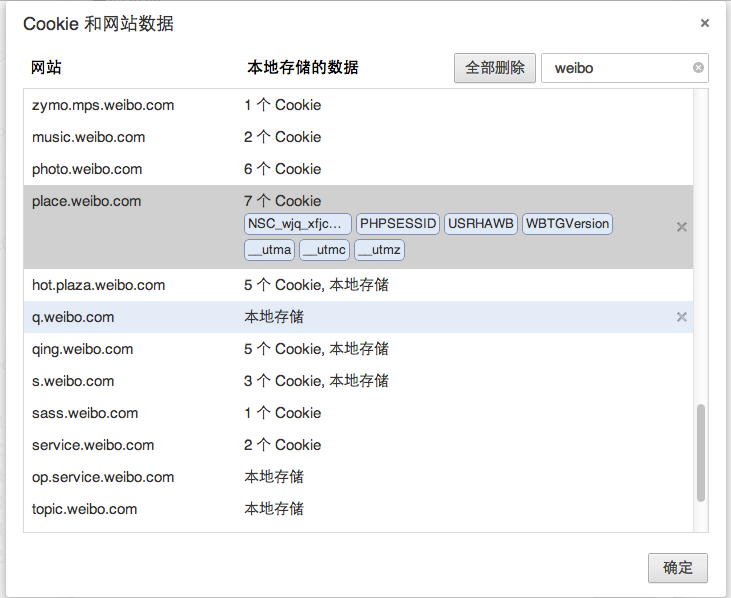
\includegraphics[width=14cm]{6.1.cookie.png}
   \label{図6.3}
   \caption{ブラウザで保存されているcookie情報}
\end{figure}

cookieには有効期限があります。有効期限の違いに従って2つに分けられます:セッションcookieと持続クッキーがあります。

もし有効期限を設定しなければ、このcookieの有効期限は新規に作成されてからブラウザを閉じるまでとなり、cookieは消滅します。このような有効期限は閲覧時のセッションのセッションcookieと呼ばれます。セッションcookieは一般的にハードディスク上には保存されず、メモリに保存されます。

もし有効期限(setMaxAge(606024))が設定されていると、ブラウザはcookieをハードディスクに保存します。ブラウザを閉じて再度開くと、これらのcookieは依然として設定された有効期限まで有効となります。ハードディスク上に保存されたcookieは異なるブラウザのプロセス間で共有することができます。たとえばIEを2つ開き、メモリに保存されたcookieに対し異なるブラウザは異なる処理方法をとります。   


